\documentclass{article}
\usepackage{iclr2027_conference,times}
\usepackage{amsmath,amssymb,booktabs,multirow,graphicx,microtype}
\usepackage{hyperref}
\usepackage{url}
\graphicspath{{../figures/}}
\newcommand{\method}{\textsc{OpenProp}}
\newcommand{\unknown}{\textsc{unknown}}
\newcommand{\obs}{\textsc{observed}}
\title{OpenProp: Language-Conditioned Entity Grounding\\under Stale, Typed Evidence}
\author{Anonymous Authors}
% Keep anonymous for submission. Do not uncomment \iclrfinalcopy.

\begin{document}
\maketitle

\begin{abstract}
An embodied agent asked for ``the mug that was beside the kettle'' must combine language with memory whose values have different types, observation times, and failure modes. We formulate current-entity grounding as an explicit typed decision. \method{} separates semantic query parsing from deterministic value-family comparators, treats unknown values as missing evidence, and discounts state observations with a replaceable persistence model trained from interval- and right-censored histories. On controlled held-out context combinations, a factorized statistical model reduces negative log-likelihood (NLL) from 1.795 to 1.239 relative to a global model and changes Top-1 grounding from 0.000 to 1.000. Frozen ablations and balanced decisions show that subject, relation, and scene factors each contribute. Under synthetic inspection-frequency confounding, interval-aware estimation improves Top-1 by 0.450 (95\% CI [0.350, 0.500]); under severe conflicting source reliability, source-specific emissions improve filtered-state NLL by 0.170 [0.166, 0.174]. On independently authored ALFRED instructions, positive lexical evidence improves train-only BM25 exact-frame accuracy by 0.124 [0.071, 0.177]. The first results validate mechanisms and the last evaluates parsing only; none establishes natural longitudinal effectiveness.
\end{abstract}

\section{Introduction}
Long-lived embodied agents must resolve entities whose recorded properties were observed at different times. A red cup may still be red while its recorded location is stale; a missing owner field says nothing about ownership; and ``beside the kettle'' has argument structure that should not collapse into unordered semantic resemblance. The target is not merely an entity compatible with a sentence, but the \emph{current} entity best supported by heterogeneous, incomplete memory.

This setting exposes three coupled problems. First, values have different semantics: numbers require tolerances, relations preserve argument identity, semantic categories permit graded comparison, and identifiers may require exactness. Second, evidence validity changes with time and context, including combinations absent from training. Third, the observation process is not the latent state process: a change discovered at an inspection occurred inside an interval, while no discovered change before a horizon is right-censoring, not a negative label.

Open-vocabulary scene graphs make instances queryable \citep{gu2024conceptgraphs,chang2023ovsg,koch2024open3dsg}; dynamic memories update scene structure or predict object locations \citep{kurenkov2023sgm,liu2024dynamem,yang2025threedmem,fan2025videoagent}. Our target is complementary: given candidates and historical observations, expose how typed match, missing coverage, confidence, and learned persistence produce a current-entity decision. We do not reconstruct geometry, select exploration actions, or replace an end-to-end memory architecture.

\begin{figure}[t]
  \centering
  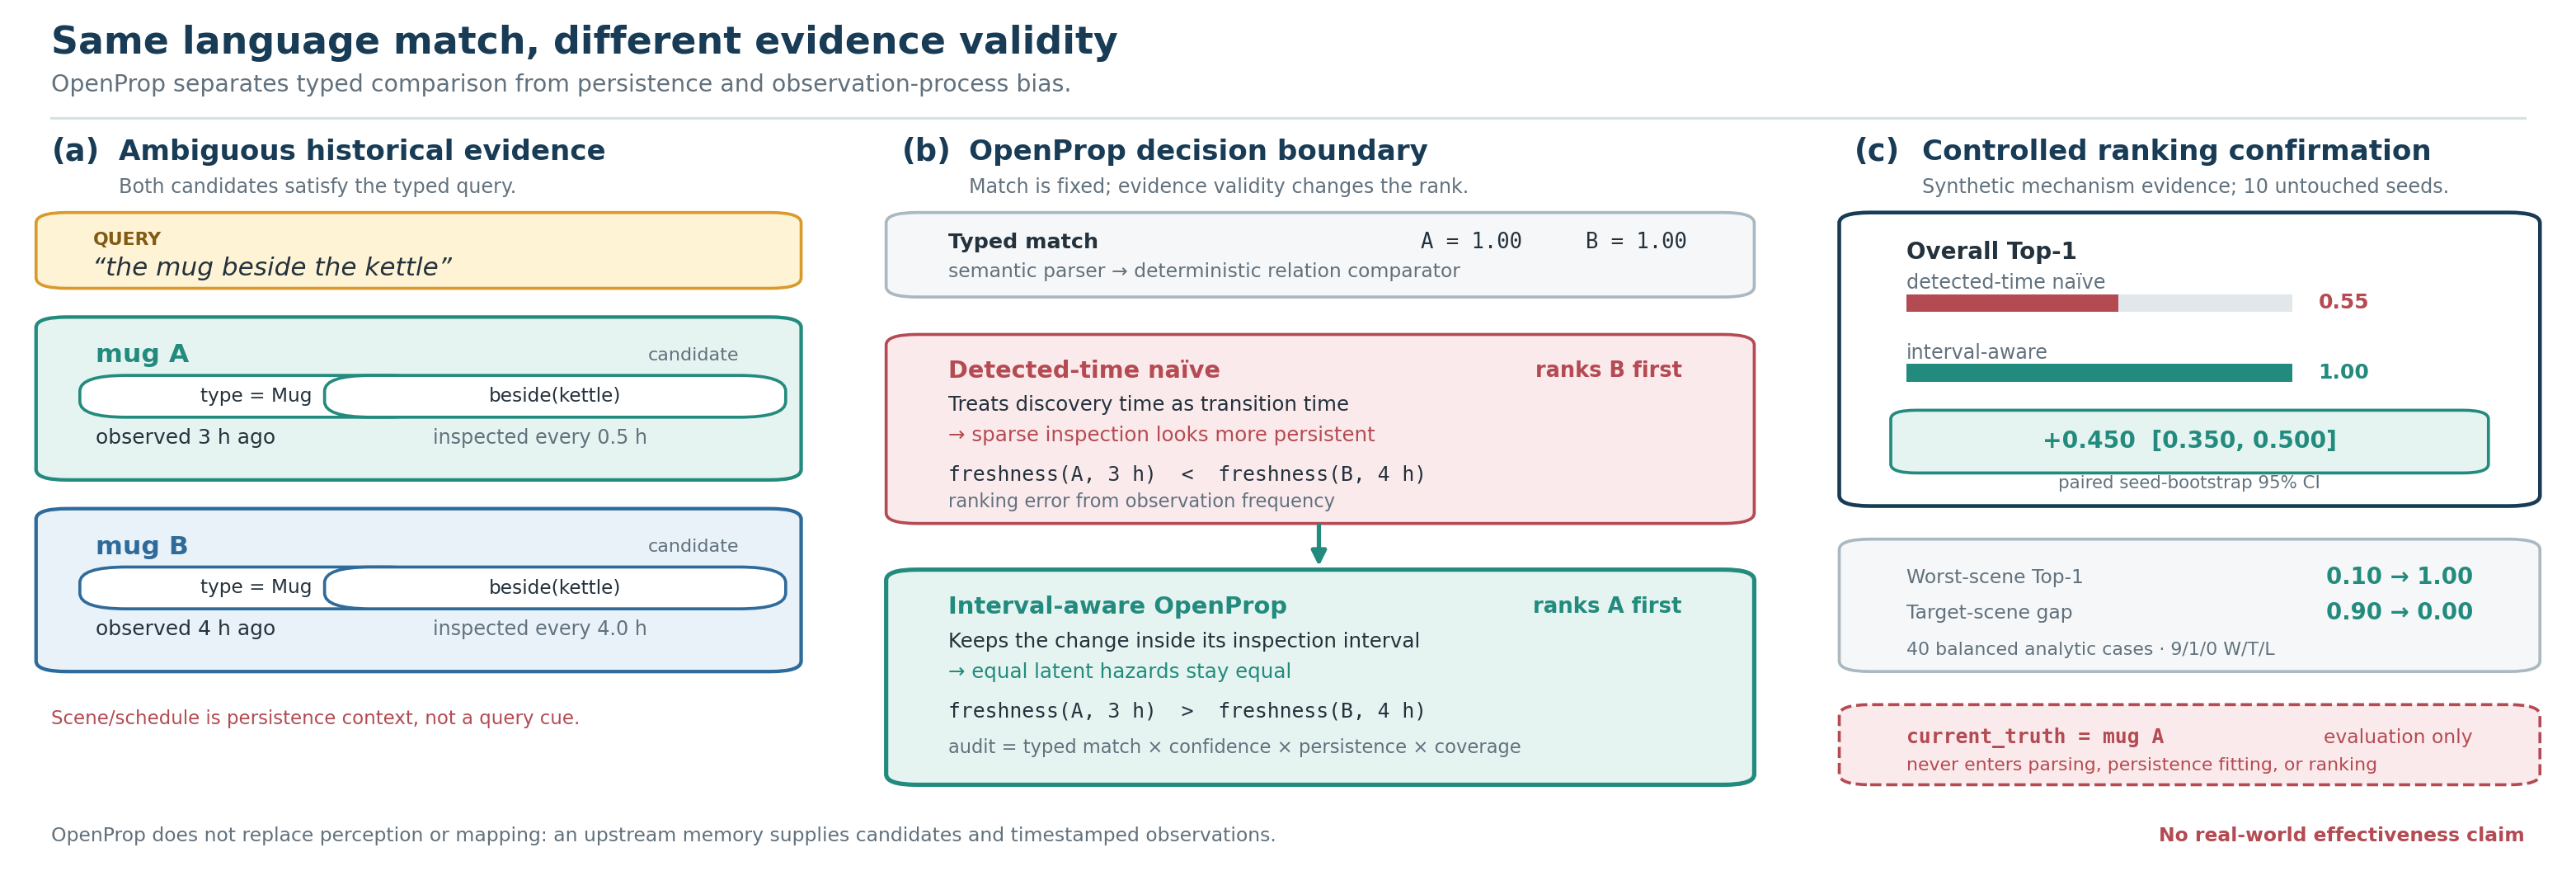
\includegraphics[width=\linewidth]{openprop_teaser.png}
  \caption{Equal typed match does not imply equal current evidence. Sparse inspection can make an identical latent process appear more persistent. The controlled confirmation reports a ranking intervention; \texttt{current\_truth} is evaluation-only.}
  \label{fig:teaser}
\end{figure}

\method{} maps language to typed constraints, compares values with registered family-specific rules, and uses survival estimates to discount state evidence. Match quality is separated from evidence coverage; timestamps, provenance, and histories remain metadata rather than comparable properties. Hidden current truth is available only to evaluation. Our contributions are: (i) an auditable typed formulation of language-conditioned current-entity grounding; (ii) a censoring-aware persistence boundary that composes typed context on unseen combinations; (iii) confirmation-split evidence connecting calibration choices to final decisions, including retained negative results; and (iv) an executable claim-to-artifact manifest. The decisive natural longitudinal evaluation remains outstanding, so our claims stop at mechanism validation and external parsing.

\section{Problem Formulation}
\paragraph{Typed memory and query.}
Let $\mathcal E=\{e_i\}_{i=1}^{N}$ be candidates supplied by an upstream memory. A registry definition $D_k$ records property $k$'s value family, aliases, optional unit, comparator, and temporal policy. The latest record is $o_{ik}=(v_{ik},z_{ik},c_{ik},s_{ik},t_{ik})$: typed value, observation state, confidence, source, and time. The state $z_{ik}\in\{\obs,\unknown,\textsc{not-applicable}\}$ separates absent evidence from mismatch. Events and histories are stored beside, not inside, the property dictionary. A hidden label $y_i(T)$ is excluded from all matcher interfaces.

A parser maps language $q$ and schema $\mathcal D$ to $Q=\{(\hat k,d_k,r_k,\tau_k)\}_{k=1}^{K}$. Registry resolution maps $\hat k$ to canonical $k$ with score $\rho_k$, giving weight $w_k=r_k\rho_k$. The parser receives no candidates or current-truth labels. Once $Q$ is fixed, scoring is deterministic.

\paragraph{Current-evidence decision.}
A typed comparator returns $m_{ik}=C_k(v_{ik},d_k;\tau_k)\in[0,1]$ and persistence returns retained support $f_{ik}(T)\in[0,1]$. Effective evidence mass is
\begin{equation}
a_{ik}=w_k\mathbf 1[z_{ik}=\obs]c_{ik}f_{ik}(T).
\end{equation}
We separate the quality of available evidence from requested evidence coverage:
\begin{equation}
M_i=\frac{\sum_k a_{ik}m_{ik}}{\sum_k a_{ik}},\qquad
C_i=\frac{\sum_k a_{ik}}{\sum_k w_k},\qquad
s_i=M_i C_i^\gamma ,
\label{eq:score}
\end{equation}
with $M_i=0$ when its denominator is zero. Thus a missing field cannot count as a mismatch, and a perfect match on one weak fragment cannot tie a fully supported candidate. Every property emits an audit record. Exact score ties use lexical entity ID, ensuring candidate-order invariance.

\section{OpenProp}
\begin{figure}[t]
  \centering
  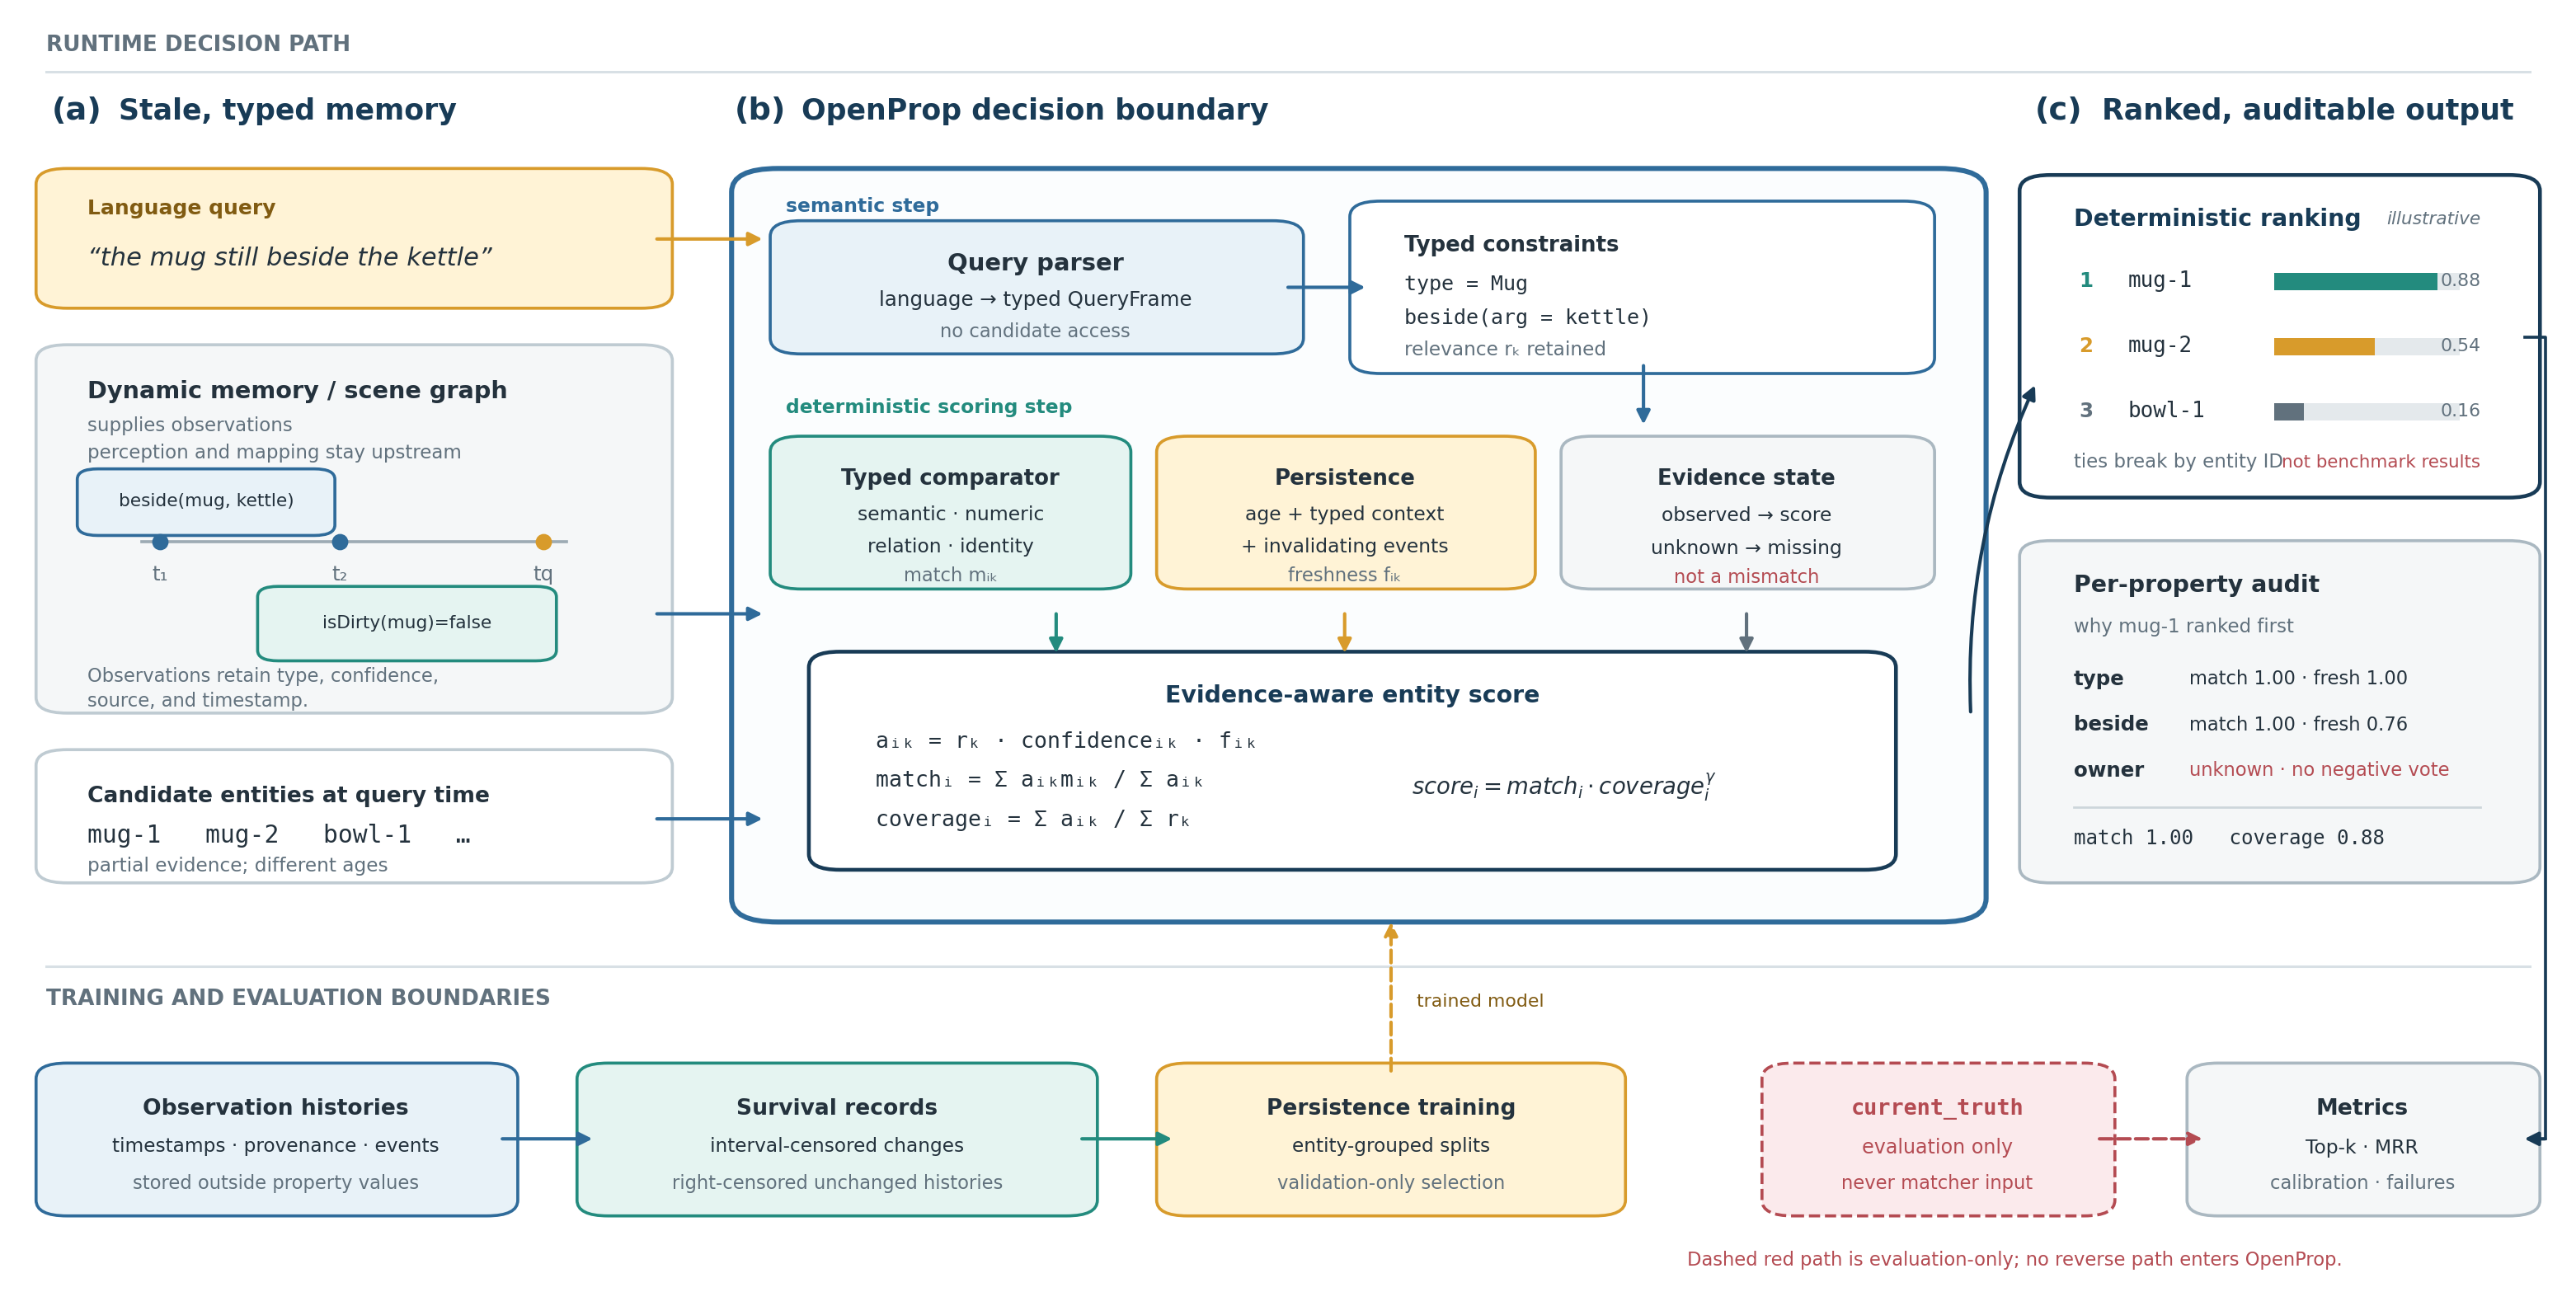
\includegraphics[width=\linewidth]{openprop_task_pipeline.png}
  \caption{The semantic boundary selects typed constraints; deterministic comparators and persistence score supplied observations. Observation histories train persistence, whereas evaluation truth never enters the ranker.}
  \label{fig:pipeline}
\end{figure}

\paragraph{Typed registries.}
\texttt{PropertyRegistry} resolves exact names and aliases before bounded fuzzy matching; schema growth is a separate opt-in operation. \texttt{ComparatorRegistry} dispatches by value family. Categorical and reference values use identity, numeric and temporal values use $\exp(-|v-d|/\tau)$, vectors use shifted cosine similarity, and relations multiply predicate similarity by the fraction of desired named arguments matched. Invalid extension outputs fail closed. Typed similarity affects only $M_i$'s numerator and cannot manufacture coverage.

\paragraph{Fixed and learned persistence.}
For age $\Delta_{ik}$ and half-life $H_k$, fixed time retention is $g_{ik}=\max(g_k^{\min},2^{-\Delta_{ik}/H_k})$. A post-observation event $e$ contributes $1-p_e(1-r_e)$. Learned models replace only $g_{ik}$ with a survival probability and retain the event product, preserving the matching contract.

Observation histories yield exact events, interval-censored changes $(l,u]$, or right-censoring at $u$. Histories are split by entity. Our main model is deliberately simple. For typed factors $x=$(property, subject type, predicate, context object, scene),
\begin{equation}
\lambda(x)=\alpha\exp\!\left(\beta_0+\sum_{j\in A}\beta_{j,x_j}\right),
\qquad S(t\mid x)=\exp[-\lambda(x)t].
\label{eq:survival}
\end{equation}
Effects are L2-regularized on training entities; a single multiplier $\alpha$ may be calibrated on validation data. Familiar factor values therefore compose on an unseen tuple. For an exact event, right-censored record, and interval-censored record, respectively, the NLL contributions are $\lambda u-\log\lambda$, $\lambda u$, and
$\lambda l-\log(1-\exp[-\lambda(u-l)])$. We compare global, smoothed exact-context, factor ablations, Weibull, Cox, and neural variants, but make no neural-architecture novelty claim.
For logged opportunities, a two-state forward likelihood uses state-specific inspection $q_0,q_1$, sensitivity $s$, and false-positive rate $f$. Positive emission probabilities are $q_0f$ before transition and $q_1s$ after transition; scaled forward--backward EM estimates the hazard and nuisance parameters from training sequences. Estimating $f$ is opt-in. For recurrent Boolean state, an optional continuous-time Markov chain replaces the one-way hazard with forward and return rates; joint EM remains training-only, and a property-specific matcher adapter fails closed on non-Boolean values. With irregular timing, each step uses its logged elapsed interval in the CTMC matrix rather than interpolating a regular grid. With multiple sources, the latent dynamics remain shared while each provenance ID receives separate inspection, sensitivity, and false-positive parameters; a tied-emission model is the direct ablation.

\paragraph{Language boundary.}
The general interface validates a schema-constrained parser output before deterministic scoring. Our ALFRED study instead uses a reproducible sparse baseline: BM25 indexes train-split human descriptions and typed frames. Positive lexical evidence may add a missing property or replace a conflicting value only when an explicit query span supports it; absent cues never delete retrieved constraints. The study ends at frame prediction and has no candidate, visual, persistence, or matcher access.

\section{Experimental Protocol}
We isolate eight executed questions rather than use success at one boundary as evidence for another; integrated longitudinal TEACh grounding remains the pending ninth question.
\textbf{Compositional persistence:} a synthetic factorized exponential generator holds out complete context tuples while every factor value remains observed. Five fixed seeds share the same test streams across models; NLL is primary, with C-index, integrated Brier score (IBS), and downstream Top-1 secondary.
\textbf{Components and decisions:} ten paired seeds omit subject, relation, or scene from the factorized model. Each three-comparison primary family uses shared paired-seed bootstrap resamples and a simultaneous maximum-deviation critical value. A separate frozen confirmation uses 40 balanced analytic crossover cases and ten untouched seeds to test whether each factor can change ranking.
\textbf{Observation process:} two strata share a true hazard of $0.25$/h but are inspected every $0.5$ or $4$ hours. We compare treating discovery time as event time against interval likelihood, first on estimation and then on frozen 40-case ranking.
\textbf{Specificity stress:} five paired seeds cross false-positive rates $\{0,.02,.05,.10\}$ and compare fixed with training-estimated specificity on shared exact test rows.
\textbf{Recurrence stress:} five paired seeds cross return rates $\{0,.15,.30,.45\}$/h and compare irreversible with joint reversible EM on independent exact-state rows; the zero-return condition is an excluded compatibility control.
\textbf{Timing stress:} five paired seeds fix 12-hour follow-up while crossing bursty gap contrasts $\{0,.50,.75,.90\}$; exact-interval EM is compared with the same outcomes on their true mean grid, and zero contrast is excluded from the primary family.
\textbf{Source-reliability stress:} five paired seeds cross source-conflict severities $\{0,.33,.67,1\}$ while holding source-average emissions fixed. Source-specific EM is compared with tied emissions on 20,000 filtered-current-state rows per seed; current truth remains evaluation-only and zero conflict is excluded from the primary family.
\textbf{External language:} ALFRED \citep{shridhar2020alfred} valid-seen and valid-unseen descriptions are parsed with train-only retrieval. Intervals are paired by case and bootstrapped by task ID, stratified by task type. No validation labels select methods. Appendix~\ref{app:protocol} gives denominators and leakage controls.

\section{Results}
\subsection{Typed composition and component decisions}
\begin{table}[t]
\centering
\caption{Held-out complete context tuples (five seeds). Mean $\pm$ std. Synthetic mechanism validation.}
\label{tab:composition}
\small
\begin{tabular}{lrrrr}
\toprule
Model & NLL$\downarrow$ & C-index$\uparrow$ & IBS$\downarrow$ & Top-1$\uparrow$\\
\midrule
Global exponential & 1.795$\pm$.033 & .500$\pm$.000 & .243$\pm$.003 & .000$\pm$.000\\
Factorized exponential & \textbf{1.239$\pm$.069} & \textbf{.749$\pm$.014} & \textbf{.079$\pm$.010} & \textbf{1.000$\pm$.000}\\
Neural compositional & 1.266$\pm$.061 & .723$\pm$.026 & .084$\pm$.009 & .972$\pm$.056\\
\bottomrule
\end{tabular}
\end{table}

Table~\ref{tab:composition} shows that typed factorization generalizes to unseen complete tuples. The statistical factorized model is stronger than the neural variant on every reported mean; the result supports structure, not neural necessity.

\begin{table}[t]
\centering
\caption{Frozen factor evidence. $\Delta$NLL is ablation minus full model; decision $\Delta$ is full minus matched ablation. Family-wise simultaneous 95\% paired-bootstrap CIs within each three-comparison family; ten seeds.}
\label{tab:components}
\small
\begin{tabular}{lrrr}
\toprule
Factor & $\Delta$NLL [sim. CI] & Decision $\Delta$ [sim. CI] & Wins\\
\midrule
Subject & .052 [.038,.066] & .347 [.329,.364] & 10/10\\
Relation & .156 [.137,.176] & .327 [.313,.340] & 10/10\\
Scene & .402 [.364,.441] & .500 [.500,.500] & 10/10\\
\bottomrule
\end{tabular}
\end{table}
All factor-ablation NLL intervals exclude zero. More importantly, Table~\ref{tab:components}'s separate balanced confirmation connects each factor to a final decision. Because cases are analytically constructed, these deltas do not estimate natural prevalence.

\subsection{Inspection bias changes entity ranking}
Treating first detection as the event time makes identical latent dynamics appear schedule-dependent. Across five seeds, the naive estimator has hazard MAE $.056\pm.004$ and a schedule gap $.074\pm.006$; interval-aware likelihood reduces these to $.006\pm.004$ and $.004\pm.004$, respectively, while improving exact-time test NLL from $2.335\pm.019$ to $2.291\pm.027$.

\begin{table}[t]
\centering
\caption{Grounding under synthetic inspection-frequency confounding. Ten untouched seeds; 40 balanced cases.}
\label{tab:inspection}
\small
\begin{tabular}{lrrr}
\toprule
Estimator & Top-1$\uparrow$ & Worst-scene$\uparrow$ & Scene gap$\downarrow$\\
\midrule
Detected-time naive & .550$\pm$.150 & .100$\pm$.300 & .900$\pm$.300\\
Interval-aware & \textbf{1.000$\pm$.000} & \textbf{1.000$\pm$.000} & \textbf{.000$\pm$.000}\\
True-hazard oracle & 1.000$\pm$.000 & 1.000$\pm$.000 & .000$\pm$.000\\
\midrule
Paired advantage [95\% CI] & +.450 [.350,.500] & +.900 [.700,1.000] & $-$.900 [$-$1.000,$-$.700]\\
\bottomrule
\end{tabular}
\end{table}
The downstream intervention (Table~\ref{tab:inspection}) demonstrates that censoring semantics can alter ranking. It does not establish effect prevalence or robustness to informative inspection, missed detections, or non-exponential dynamics.

\subsection{External language parsing}
\begin{table}[t]
\centering
\caption{ALFRED language-to-frame parsing. The hybrid adds only positive span evidence to train-only BM25. Task-clustered 95\% CIs are shown for exact-frame deltas.}
\label{tab:alfred}
\small
\begin{tabular}{llrrr}
\toprule
Split & Method & Property F1 & Value recall & Exact frame\\
\midrule
Seen (487) & Evidence only & .788 & .652 & .345\\
 & BM25 & .983 & .818 & .612\\
 & BM25 + evidence & \textbf{.989} & \textbf{.880} & \textbf{.710}\\
 & $\Delta$ vs BM25 & +.006 & +.062 & +.099 [.064,.134]\\
\midrule
Unseen (458) & Evidence only & .822 & .697 & .404\\
 & BM25 & .979 & .802 & .611\\
 & BM25 + evidence & \textbf{.986} & \textbf{.896} & \textbf{.736}\\
 & $\Delta$ vs BM25 & +.006 & +.094 & +.124 [.071,.177]\\
\bottomrule
\end{tabular}
\end{table}
Positive-evidence fusion improves all three measures on both splits (Table~\ref{tab:alfred}); all task-clustered delta intervals exclude zero. This is independently authored language but only a frame-prediction result. It supplies no visual, temporal, or end-to-end grounding evidence.

\subsection{False-positive observation stress}

A paired specificity stress adds false-positive emissions to the training-only observation EM. At false-positive rate .10, estimating specificity reduces hazard MAE from .0284 to .0061 and improves exact-test NLL in 5/5 seeds by .00615 [.00343,.00887], with a family-wise simultaneous interval across three nonzero rates. At .02 and .05 the intervals cross zero, so extra noise estimation is not claimed to help universally.
\subsection{Recurrent-state observation stress}
At return rates .15, .30, and .45/h, reversible EM improves exact-state NLL over irreversible EM by .06038 [.05016,.07060], .08099 [.07314,.08884], and .08263 [.07560,.08965]. All three simultaneous intervals exclude zero and every condition wins in 5/5 paired seeds. At zero return, NLL is .46056 versus .46061, a compatibility near-tie rather than an equivalence claim. This validates a matched binary regular-grid mechanism, not real-world recurrence.

\subsection{Irregular observation-timing stress}
At bursty gap contrasts .50, .75, and .90, exact-interval EM improves current-state NLL over mean-grid EM by .00391 [.00151,.00630], .01446 [.01217,.01675], and .03140 [.02907,.03373]. All simultaneous intervals exclude zero and every condition wins in 5/5 seeds; the regular-grid control differs by .00001. This holds follow-up and mean interval fixed and validates exogenous two-gap timing, not natural observability.

\subsection{Conflicting source-reliability stress}
At conflict severities .33, .67, and 1.00, source-specific emissions improve filtered-current-state NLL over tied emissions by .02173 [.02059,.02287], .08235 [.07978,.08492], and .17006 [.16565,.17447]. All simultaneous intervals exclude zero and every condition wins in 5/5 seeds. At zero conflict, NLL is .29595 versus .29591, a compatibility near-tie. Because source-average emissions and observation budgets are fixed, the result isolates source heterogeneity, but only for two conditionally independent stationary sources.

\subsection{Retained negative and pending evidence}
A favorable average is insufficient when the proposed explanation or deployment claim fails a targeted test. Table~\ref{tab:boundaries} therefore makes three boundaries part of the result rather than relegating them to implementation notes. First, the neural persistence model does not justify an architectural novelty claim: it is weaker than typed factorization on all four controlled means. Second, calibration-only adaptation is not generally safe. Under a development stress test with 20\% corrupted evidence, repetition reduces noisy control activations from 2/10 to 0/10, yet affected C-index changes by $-$.036 (95\% bootstrap lower bound $-$.109; worst seed $-$.363). The intervention changes whether adaptation activates, not whether the resulting update is valid. Third, the integrated longitudinal result remains pending.

\begin{table}[t]
\centering
\caption{Claims excluded or pending after adversarial evaluation.}
\label{tab:boundaries}
\small
\begin{tabular}{p{.24\linewidth}p{.15\linewidth}p{.45\linewidth}}
\toprule
Candidate claim & Status & Frozen evidence and consequence\\
\midrule
Neural persistence is necessary & Contradicted & Factorized vs. neural NLL: 1.239 vs. 1.266; Top-1: 1.000 vs. .972. Claim typed factorization, not neural novelty.\\
Semi-real longitudinal effectiveness & Pending & No official TEACh longitudinal result is available; no performance wording is allowed.\\
Calibration-only adaptation is generally safe & Contradicted & Under 20\% flips, affected C-index changes $-$.036 (lower bound $-$.109; worst seed $-$.363). Report an identifiability boundary.\\
\bottomrule
\end{tabular}
\end{table}

\subsection{Frozen longitudinal protocol}
The missing integrated experiment is not an unspecified future benchmark. We freeze a TEACh \citep{padmakumar2022teach} protocol designed to prevent action outcomes from leaking into the decision. Candidates must be visible at least once strictly before the recorded target action. The action-time state difference, final state, target identity, and all post-decision observations are excluded. Floorplans, rather than frames, define train and evaluation separation. The same all-case denominator must retain target-unobserved, parse-failure, type-unique, and same-type-ambiguous cases; impossible cases may be reported as slices but not silently filtered.

The automatic frame supplies only a target-type condition and is not called a complete semantic oracle. A richer-frame condition requires three annotators to see only Commander text, fixed target type, and the allowed typed state vocabulary. Every attribute requires an exact text span. Candidate properties, timestamps, outcomes, final truth, and model outputs remain hidden. Two-of-three deterministic majority and a predeclared 0.80 pairwise exact semantic-agreement gate are required before evaluation. The protocol compares full typed persistence with property-only, fixed-decay, no-freshness, and language-oracle boundaries, reporting Top-1, coverage-conditioned performance, abstention curves, and candidate-recall ceilings. Until these gates pass, the experiment contributes no quantitative claim.


\section{Related Work}
ALFRED and TEACh \citep{shridhar2020alfred,padmakumar2022teach} motivate references tied to changing household scenes, but end-task metrics do not isolate parsing, candidate recall, stale evidence, and control. Open-vocabulary representations \citep{gu2024conceptgraphs,chang2023ovsg,koch2024open3dsg} address perception and contextual retrieval; dynamic memories \citep{kurenkov2023sgm,liu2024dynamem,yang2025threedmem,fan2025videoagent} address scene updates and persistent reasoning. \method{} consumes supplied candidates and histories but isolates a typed, decomposable current-evidence score. Survival methods model censored event times and calibration \citep{lee2018deephit,avati2020survivalcrps}; our contribution is not a new censoring objective, but its placement behind an auditable typed grounding interface and measurement of when estimation changes rank.

\section{Discussion, Limitations, and Conclusion}
\paragraph{What the evidence establishes.}
The supported contribution is an explicit current-evidence boundary. Typed factorization, not model capacity, carries the controlled compositional result. Interval-aware training prevents inspection schedule from becoming a false ranking cue, specificity estimation removes a high-false-positive bias while retaining lower-noise ties, and a reversible binary CTMC handles return transitions, logged irregular intervals, and source-specific reliability with near-tie controls. The negative results are equally important: neural necessity is contradicted; noisy calibration evidence does not certify safe adaptation; and ALFRED stops at parsing.

\paragraph{Statistical and task limitations.}
Current evidence does not establish naturalistic longitudinal effectiveness. Synthetic generators align with the statistical model, and balanced cases are stress tests rather than prevalence estimates. The main exponential hazard assumes irreversible transitions and proportional typed effects; the optional recurrent model covers only a binary Markov state with known initial state. Its irregular experiment uses exogenous two-gap schedules, not informative timing or timestamp error. Its source experiment assumes two stable, conditionally independent sources and does not cover correlated, adversarial, appearing, or disappearing sources. Real histories may contain multi-valued dynamics, nonstationarity, and unseen interactions. The specificity stress uses one homogeneous detector and separates from fixed specificity only at the largest tested rate. ALFRED is independently authored but templated and contains train--validation query overlap; duplicate-preserving evaluation prevents inflated edit gains but does not make it an open-domain parsing benchmark.

\paragraph{System boundary.}
Candidate recall, cross-time identity, perception, map consistency, and synchronization remain upstream. A transparent score cannot recover an entity that was never observed or repair an identity merge using evaluation truth. The coverage term is a decision signal rather than proof of correctness; a deployment should expose unobserved targets, ties, provenance gaps, unsupported factor values, and declared backoff. Because the matcher is deterministic after parsing, these channels can be audited without conflating them with language-model variability.

\paragraph{Broader impact.}
Freshness can amplify unequal observation coverage: frequently monitored places, people, or object classes may appear more current for operational rather than semantic reasons. Systems should preserve provenance, report coverage and source-stratified behavior, avoid collecting socially sensitive properties without a legitimate task basis, and permit abstention, correction, and deletion. The explicit decomposition supports such audits but cannot make inappropriate sensing fair.

\paragraph{Conclusion.}
In summary, \method{} formulates current-entity grounding as a typed decision under incomplete and stale evidence. It keeps unknown values missing, current truth outside the matcher, and every score auditable. Controlled experiments establish compositional, factor-specific, and censoring-aware mechanisms; external language data supports the parsing boundary only. A floorplan-disjoint longitudinal experiment with independently held current truth is the decisive next test.
\label{sec:main-end}

\section*{AI Use Statement}
Generative AI systems were used to assist with code implementation, experiment orchestration, prose drafting and editing, and formatting. Machine-generated changes were checked through executable tests and claim-to-artifact manifests. Final scientific responsibility remains with the authors.

\section*{Ethics Statement}
Freshness scores can reflect unequal monitoring rather than semantics and may amplify observation bias. The method therefore preserves provenance, time, missing coverage, and per-property audits. Applications should avoid collecting socially sensitive properties without a legitimate task basis and should support abstention, correction, and deletion. Auditability exposes these risks but does not make the underlying observations fair or appropriate.

\section*{Reproducibility Statement}
The anonymous supplement contains deterministic table builders, fixed seeds, executable claim checks, artifact hashes, and tests for typed values, unknown semantics, current-truth isolation, and candidate-order invariance. Appendix~\ref{app:protocol} specifies denominators, splits, uncertainty, and claim boundaries. The official longitudinal result is not represented as complete.

\bibliography{references}
\bibliographystyle{iclr2027_conference}

\appendix
\small
\section{Detailed Protocol and Claim Boundaries}
\label{app:protocol}
\paragraph{Controlled composition.}
Training and test are generated independently per seed. Complete context tuples are disjoint, but each factor value appears in training. All models share test rows. Five seeds report mean and standard deviation; the component confirmation uses ten predeclared paired seeds and family-wise simultaneous intervals within each three-comparison primary family. NLL is primary. Synthetic results validate the declared mechanism only.

\paragraph{Decision confirmation.}
Each factor uses 40 analytic confidence--age crossover cases, balanced between old and new targets. The full and factor-removal models see identical histories and cases. The confirmation seeds were untouched after protocol freeze. Lexical entity ID resolves exact score ties, and permutation tests check candidate-order invariance.

\paragraph{Observation-process intervention.}
Both scene strata have hazard $0.25$/h and differ only in inspection interval. Each seed uses 600 histories per scene for estimation. Estimation uses no downstream labels. Ranking pairs a 3-hour target observation with a 4-hour distractor and balances target scene. Scene is persistence context, never a queried property. The one Top-1 tie seed is retained.

\paragraph{Specificity stress.}
Five paired seeds use false-positive rates $\{0,.02,.05,.10\}$, 1,200 training sequences, and 1,000 independent exact-time test rows per condition. Training transition draws and test rows are shared across rates. One EM fit fixes specificity at one and the other estimates false-positive rate from training sequences only. The primary nonzero-rate NLL family uses shared paired-seed resamples and a simultaneous maximum-deviation critical value. At .10 the interval excludes zero; at .02 and .05 it does not.

\paragraph{Recurrence stress.}
Five paired seeds use forward rate .30/h, return rates $\{0,.15,.30,.45\}$/h, 600 training sequences, and 2,000 independent exact-state rows per condition. Training streams and test horizon/outcome uniforms are paired across conditions. Joint EM sees observation outcomes only. The three nonzero irreversible-minus-reversible NLL comparisons use 20,000 shared seed resamples and simultaneous maximum-deviation intervals; zero return is excluded from that family.

\paragraph{Timing stress.}
Five paired seeds fix each episode at 16 opportunities and 12 hours, with fourteen short and two long gaps in a paired random order. Contrasts $\{0,.50,.75,.90\}$ preserve the .75-hour mean. Each condition uses 600 training episodes and 20,000 shared exact-state test rows. The three nonzero mean-grid-minus-exact NLL comparisons use 20,000 shared seed resamples and simultaneous intervals; zero contrast is excluded.

\paragraph{Source-reliability stress.}
Five paired seeds use two sources, 400 training episodes, 24 half-hour opportunities, and 20,000 filtered-current-state test rows per severity. Severity moves source inspection, sensitivity, and false-positive parameters symmetrically in opposite directions while their averages remain fixed. Latent training paths are discarded; evaluation state paths are paired and withheld from both filters. The three nonzero tied-minus-source-specific NLL comparisons use 20,000 shared seed resamples and simultaneous intervals; zero conflict is excluded.

\paragraph{ALFRED language boundary.}
The official train split alone forms the BM25 index. Evaluation includes all 487 valid-seen and 458 valid-unseen descriptions in the frozen selection. Retrieval ties use lexical training-case ID. Exact duplicate queries retain the retrieved frame unchanged. The positive-evidence layer has no access to candidate entities, observations, persistence, matcher scores, or validation labels. Bootstrap resampling is clustered by ALFRED task ID and stratified by task type.

\paragraph{Outstanding longitudinal test.}
The frozen TEACh protocol \citep{padmakumar2022teach} requires floorplan-disjoint histories and candidates visible strictly before the target action; action-time state differences and final state are excluded from matching. Reports must retain type-unique, same-type ambiguous, target-unobserved, and parse-failure slices on the all-case denominator. Richer referential attributes require independently annotated text spans and a predeclared agreement gate. These results are pending and therefore absent from the main claims.

\end{document}
